% ============================================================
% Return-Sharpe Aware Ranking with Multi-Model RRF Fusion
% Overleaf编译方式：菜单→Compiler→XeLaTeX
% ============================================================

\documentclass[11pt,a4paper]{ctexart}

\usepackage{amsmath,amssymb,amsfonts}
\usepackage{booktabs}
\usepackage{multirow}
\usepackage{graphicx}
\usepackage{pgfplots}
\pgfplotsset{compat=1.18}
\usepackage{tikz}
\usetikzlibrary{patterns,calc}
\usepackage{xcolor}
\usepackage{hyperref}
\hypersetup{colorlinks=true,linkcolor=blue,citecolor=blue}
\usepackage[margin=2.5cm]{geometry}
\usepackage{enumitem}
\usepackage{caption}
\usepackage{subcaption}
\usepackage{array}
\usepackage{colortbl}
\usepackage{fancyhdr}

\definecolor{bestval}{RGB}{0,128,0}
\definecolor{secondval}{RGB}{0,0,180}
\definecolor{worstval}{RGB}{180,0,0}
\newcommand{\best}[1]{\textcolor{bestval}{\textbf{#1}}}
\newcommand{\second}[1]{\textcolor{secondval}{#1}}

\pagestyle{fancy}
\fancyhf{}
\fancyhead[L]{\small Return-Sharpe Aware Ranking with Multi-Model RRF Fusion \hspace{1em} A PREPRINT}
\fancyfoot[C]{\thepage}
\renewcommand{\headrulewidth}{0pt}

\title{\LARGE Return-Sharpe Aware Ranking with Multi-Model RRF Fusion\\[0.3em]
\large for Quantitative Stock Selection\\[1em]
\normalsize A PREPRINT}
\author{
\textbf{Zheng Luo} \hspace{2em} [Co-author Name]\\[0.3em]
\small School of Computer Science \hspace{2em} School of Economics and Business\\
\small Chongqing University \hspace{2em} Chongqing University\\
\small Chongqing, China \hspace{2em} Chongqing, China\\[0.3em]
\small \texttt{luozheng@cqu.edu.cn} \hspace{2em} \texttt{[email@cqu.edu.cn]}
}
\date{2026年5月26日}

\begin{document}
\maketitle
\thispagestyle{fancy}

% ============================================================
% Abstract
% ============================================================
\begin{center}
\textbf{\large ABSTRACT}
\end{center}
\vspace{-0.5em}

量化选股策略的核心是以算法代替主观判断，筛选具有超额收益潜力的股票并构建最优的投资组合。传统多因子选股方法存在两个关键局限：一是损失函数未能直接对齐投资目标，同时过度依赖历史有效的高收益、低风险，形成路径依赖；二是单模型预测稳定性不足，且模型从数据中自动学习规律和相关性而决策逻辑高度抽象从而缺乏可解释性。针对这些不足，本研究提出一种融合收益-夏普感知排序损失与递归排名融合的多模型量化选股框架，并系统对比四种排序策略，给出实际应用建议。基于近10年约2500只A股周频数据的实证研究表明，CVaR感知损失函数（E1c）有效提升了风险调整后收益，夏普比率从基线LightGBM的0.492提升至0.592，年化收益率达15.90\%；然而，多模型融合策略的整体表现不佳，受XGBoost基线模型负收益（年化$-$14.29\%）拖累，多数融合方法出现负收益，仅Stacking融合（E2c）保持正收益（年化7.19\%）。配对检验显示0/15组差异显著，表明当前测试期100周样本量偏小，统计检验功效不足。本研究诚实报告了上述发现，并讨论了方法局限性与未来改进方向。

\vspace{1em}
\noindent\textbf{Keywords} \hspace{0.5em} 排序学习·收益感知损失·RRF多模型融合·可解释AI

\vspace{1.5em}

% ============================================================
% 1 Introduction
% ============================================================
\section{Introduction}

现在量化交易的策略，是使用先进的机器学习模型来广泛寻找金融市场中的有机会的投资机会，其中关键的任务便是排序。正确的排序帮助决策资金在股票间的分配，并最终决定了投资组合的利润和风险。

近年来，深度学习技术在量化投资领域取得了显著进展。基于Transformer架构的时序模型和LSTM等循环神经网络，凭借强大的非线性拟合能力，在股价预测、因子挖掘等任务中展现出潜力。然而，将深度学习直接应用于A股量化选股仍面临三大根本性挑战。其一，过拟合风险突出。金融数据的信噪比极低，有效信号被海量噪声所淹没，而深度学习模型参数量巨大，极易将噪声误认为信号进行学习，导致测试集表现完美但实盘表现崩塌的"过拟合陷阱"。其二，训练成本与收益不匹配。在A股周频数据的小数据场景下（约2500只股票$\times$500周$\approx$150万条样本），深度学习模型的训练成本高、收敛不稳定，且对超参数和随机种子高度敏感，难以保证结果的可复现性。其三，可解释性严重不足。深度学习作为典型的黑箱模型，其内部决策逻辑高度抽象，无法提供因子贡献分解或信号来源追溯，难以满足投资决策的透明性需求和合规审查要求。上述问题使得基于排序学习（LTR）与树模型的路线成为更务实的选择：树模型参数少、不易过拟合，训练速度快且结果稳定，且天然具备可解释性——能够通过特征重要性和SHAP值清晰揭示每个预测的驱动因素。LTR+树模型路线的核心优势在于，在可解释性与预测性能之间取得了工程上可落地的平衡：既避免了深度学习的过拟合和黑箱问题，又通过排序学习框架保证了足够的预测能力，使得模型输出既"可信"又"可解释"。

传统多因子选股模型的核心思想是，通过构建一系列能够预测股票未来收益的因子，如价值因子、成长因子等，依据各因子进行线性加权打分并排序，后构建投资组合。这种方法的逻辑在于，不同因子从不同维度刻画了股票的收益特征，通过多维度信息的整合，可以获得比单一指标更稳健的股票评估。传统多因子选股模型，如等权加权或线性回归方法，因实现简单、可解释性强，且在过去的实践中创造了超额收益，成为中国A股市场量化投资的主流框架。

然而，这种传统方法在理论上存在局限，首先是损失函数与优化目标错位。用OLS或简单的排序损失训练模型，容易忽视投资组合的实际风险调整后收益，导致模型可能选入夏普比率较低的股票；其次，单模型预测存在系统性偏差。金融时间序列具有高度噪声、非平稳性等特征，不同的模型对数据的假设不同，其预测误差则会出现相应的异质性，导致难以在不同市场环境下保持稳定；最后是模型决策缺乏可解释性。多因子选股逐渐演变为"黑箱"操作，而这样的模型输出难以满足对决策透明度的要求和帮助合风险控制。

针对上述问题，本文提出一种融合模型。首先，设计了一种将未来收益预期与历史波动率嵌入排序损失函数的优化目标，通过收益加权NDCG和夏普惩罚项引导模型优先学习高收益低波动个股的特征；其次，采用RRF算法对LightGBM和XGBoost等多个差异化基础排序模型的输出进行融合，并引入大语言模型（LLM）生成选股决策的自然语言解释，提升策略透明度。

为验证该框架的有效性，我们在A股市场设计了四组核心实验：对比标准LambdaRank与收益-夏普感知损失函数，验证改进损失函数的有效性；评估分数平均、RRF、Stacking及加权RRF四种融合策略，证明RRF融合的优越性；测试纯模型输出与LLM增强解释方案，验证AI解读的实用价值；系统对比Pointwise、Pairwise、Listwise及本文方法的综合表现。实验中包含基线对比和消融实验，以验证各创新组件的独立贡献。基于近10年约2500只A股周频数据的实证研究表明，CVaR感知损失函数（E1c）将夏普比率从基线的0.492提升至0.592，年化收益率达15.90\%；然而，多模型融合策略受XGBoost基线模型负表现拖累，整体效果不及预期，仅Stacking融合保持正收益。配对检验显示0/15组差异显著，表明当前测试期样本量偏小，统计检验功效不足，需更长时间窗口验证。

这项研究贡献了一个面向A股市场的收益感知排序损失与多模型融合的综合基准，揭示了不同损失函数设计和融合策略如何影响模型学习横截面和时间模式的能力。通过阐明损失函数选择、模型融合与投资组合性能之间的关系，本研究为开发更有效的量化金融深度学习模型提供了更清晰的方向。

% ============================================================
% 2 Experiment Preparation
% ============================================================
\section{Experiment Preparation}

\subsection{Data Description}

数据来源与样本划分：本实验使用akshare提供的A股日线前复权数据作为研究样本，股票池为2016年前上市且未退市的A股，约2589只。时间范围从2014年1月到2024年12月。

特征与标签：按照时间顺序将数据集划分为训练集、验证集和测试集三部分。数据集划分严格遵循时间顺序，避免未来信息泄露，确保实验结果的可靠性。训练集为2014-01至2020-12（766,196行，2,257只股票），用于模型参数学习；验证集为2021-01至2022-12（232,150行），用于超参数调优和早停策略；测试集为2023-01至2024-12（225,566行，100个调仓周），用于最终模型性能评估。

因子数量为52个（排除group\_id/group\_size和6个全零因子），缺失值用列内中位数填充。

% ============================================================
% 3 Experiment
% ============================================================
\section{Experiment}

% ============================================================
% 3.1 收益-夏普感知损失函数对比
% ============================================================
\subsection{收益-夏普感知损失函数对比}

标准LambdaRank损失函数通过优化NDCG指标来提升排序质量，其核心思想是使模型输出的排序与真实收益排序尽可能一致。然而，从投资组合管理的角度看，排序准确性并非唯一目标——投资决策的核心是判断选入Top-K组合的股票能否带来较高的收益和风险调整能力。标准NDCG在实盘中存在两个局限性：收益权重缺失。它对高收益股票和低收益股票给予相同的排序权重，不能区分不同收益水平的股票对投资组合的贡献差异；风险考量不足。未考虑股票的波动率特征，可能导致选入高收益但高波动的股票，从而降低投资组合的夏普比率。

针对上述问题，本实验设计了改进标签的构造方法，逐步将投资目标嵌入排序学习过程。

\subsubsection{实验原理}

本文设计了四种不同的排序损失函数，用于对比不同目标函数对选股策略绩效的影响，具体形式如下：

\textbf{1. 标准NDCG损失（Baseline）}

标准NDCG损失仅优化排序质量，不考虑收益与风险特征，其数学形式为：
\begin{equation}
L_{\text{rank}} = -\frac{1}{|D_q|} \sum_{k=1}^{K} \frac{2^{rel_k} - 1}{\log(k+1)}
\end{equation}
其中$rel_k$为离散相关性标签（取值范围为0--30的整数）。

\textbf{2. 收益加权NDCG损失（E1a）}

在标准排名标签基础上，根据实际收益率大小额外提升高收益股票的权重，引导模型更侧重将高收益股票排在Top-K区间。增益函数定义为：
\begin{equation}
g(r_k) = |r_k|^{\alpha} \cdot \text{sign}(r_k)
\end{equation}
其中$r_k$为第$k$只股票的未来一周收益率，$\alpha$为收益敏感度参数，本文默认设置$\alpha = 1.0$。对应损失函数为：
\begin{equation}
L_{\text{return}} = -\frac{1}{|D_q|} \sum_{k=1}^{K} \frac{g(r_k)}{\log(k+1)}
\end{equation}

\textbf{3. 收益加权+夏普惩罚（E1b）}

在E1a基础上引入波动率惩罚项，降低高波动股票的权重，目标是提升组合的风险调整后收益。夏普惩罚项定义为：
\begin{equation}
L_{\text{sharpe}} = L_{\text{return}} + \lambda \cdot \max(0, -\text{Sharpe}_{\text{TopK}})
\end{equation}
其中$\text{Sharpe}_{\text{TopK}}$为Top-K组合的滚动夏普比率，$\lambda$为惩罚系数，本文默认设置$\lambda = 0.5$。

\textbf{4. 收益加权+夏普惩罚+CVaR约束（E1c）}

在E1b基础上进一步引入条件风险价值（CVaR）约束，对极端亏损风险进行额外惩罚，避免策略选入可能发生极端亏损的股票。CVaR约束项定义为：
\begin{equation}
L_{\text{cvar}} = L_{\text{sharpe}} + \gamma \cdot \text{CVaR}_{\alpha}(\text{TopK})
\end{equation}
其中$\text{CVaR}_{\alpha}$为Top-K组合在置信水平$\alpha$下的条件风险价值，本文默认设置$\alpha = 0.90$；$\gamma$为风险厌恶系数，本文默认设置$\gamma = 0.3$。

\subsubsection{实验过程}

\textbf{1. 模型训练}

采用LightGBM作为基础模型，设置五组对比实验：

\begin{table}[htbp]
\centering
\caption{实验1：实验组设计}
\label{tab:exp1-groups}
\begin{tabular}{lll}
\toprule
\textbf{组别} & \textbf{损失函数} & \textbf{说明} \\
\midrule
B-LGBM & 标准LambdaRank (NDCG) & LightGBM默认lambdarank目标 \\
B-XGB  & 标准rank:ndcg & XGBoost默认rank:ndcg目标 \\
E1a    & 收益加权NDCG & 增益函数替换为连续收益率加权 \\
E1b    & 收益加权NDCG + 夏普惩罚 & 加入Top-K组合夏普比率惩罚项 \\
E1c    & 收益加权NDCG + 夏普惩罚 + CVaR & 加入条件风险价值约束 \\
\bottomrule
\end{tabular}
\end{table}

训练参数设置：LightGBM采用objective=lambdarank、metric=ndcg、early\_stopping=100，通过Optuna进行20轮超参数搜索；XGBoost采用objective=rank:ndcg、early\_stopping=20，同样通过Optuna进行20轮超参数搜索。

\textbf{2. 核心代码实现}

本研究实现了三个层次递进的标签构造函数，以增强模型对风险调整后收益的学习能力：

\begin{itemize}
\item 第一层为\texttt{return\_aware\_relevance}（对应实验组E1a）：在标准排名标签基础上，根据实际收益率大小动态提升高收益股票的标签值，引导模型更关注具有超额收益潜力的资产。
\item 第二层为\texttt{sharpe\_aware\_relevance}（对应实验组E1b）：在E1a基础上引入波动率惩罚机制，通过夏普惩罚系数（本文设置为0.5）对高波动股票的标签进行调整，引导模型平衡收益与风险。
\item 第三层为\texttt{cvar\_aware\_relevance}（对应实验组E1c）：在E1b基础上加入CVaR（条件风险价值）惩罚项，在置信水平为0.10下对左尾极端收益股票施加额外惩罚（惩罚系数设置为0.3），增强模型对下行风险的敏感性。
\end{itemize}

为支持灵活的标签策略实验，本研究实现了\texttt{train\_final\_lightgbm\_with\_label\_fn}函数作为统一训练入口，允许传入任意自定义标签构造函数完成模型训练。

\subsubsection{实验结果}

% ---- 填充真实数据 ----

\textbf{1. 排序质量对比}

\begin{table}[htbp]
\centering
\caption{实验1：排序质量与回测指标对比}
\label{tab:exp1-ndcg}
\begin{tabular}{lccccc}
\toprule
\textbf{方法} & \textbf{NDCG@10} & \textbf{年化收益(\%)} & \textbf{夏普比率} & \textbf{最大回撤(\%)} & \textbf{最优vol\_pen.} \\
\midrule
B-LGBM (基线)       & 0.1549 & 13.80 & 0.492 & 17.56 & 5.0 \\
E1a (收益加权)       & \second{0.2057} & 9.92 & 0.369 & 19.41 & 5.0 \\
E1b (收益+夏普)      & 0.1479 & 13.71 & 0.532 & \best{13.94} & 3.0 \\
E1c (收益+夏普+CVaR) & 0.1378 & \best{15.90} & \best{0.592} & 16.03 & 3.0 \\
\bottomrule
\end{tabular}
\end{table}

实验结果表明，收益-夏普感知损失函数有效提升了风险调整后收益。E1c-LGBM夏普比率达到0.592，优于基线B-LGBM的0.492，年化收益达15.90\%；E1b-LGBM最大回撤降至13.94\%，为所有方法中最低，验证了夏普惩罚项对波动率控制的有效性。然而，NDCG@10排序质量与回测表现呈现反向关系：E1a的NDCG@10最高（0.2057）但夏普比率并非最优（0.369），E1c的NDCG@10最低（0.1378）但夏普比率最高（0.592），表明排序准确性并不直接等价于投资绩效。

\textbf{2. vol\_penalty参数敏感性分析}

实验1中各方法的最优vol\_penalty配置如下：B-LGBM和E1a-LGBM均在vol\_penalty=5.0时取得最优夏普比率，而E1b-LGBM和E1c-LGBM在vol\_penalty=3.0时表现最优。引入风险感知标签后模型自身已具备波动率筛选能力，无需过高的外部波动率惩罚，因此最优vol\_penalty从5.0降至3.0。

% ============================================================
% 3.2 多模型排序融合对比
% ============================================================
\subsection{多模型排序融合对比}

单模型预测存在系统性偏差。金融时间序列具有高度噪声、非平稳性和regime switching等特征，不同模型对数据生成过程的假设不同，其预测误差在不同时期和不同市场状态下呈现异质性，使得单一模型难以在所有市场环境下保持稳定表现，而简单模型平均又无法充分利用各模型的比较优势。为解决上述预测稳定性不足和排序尺度差异的问题，本实验设计了四种多模型融合策略，通过排序级融合提升选股稳定性。

\subsubsection{实验原理}

\textbf{1. 分数平均融合（E2a）}

将多个模型的预测分数归一化后取平均，生成融合排序，核心思想是通过平均降低单模型预测方差，但依赖于分数归一化处理。融合分数计算公式如下：
\begin{equation}
s_{\text{fusion}} = \frac{1}{M} \sum_{m=1}^{M} \text{norm}(s_m)
\end{equation}
其中$s_m$为模型$m$的预测分数，$\text{norm}(\cdot)$为归一化函数，$M$为模型数量。

\textbf{2. RRF融合（E2b）}

Reciprocal Rank Fusion（RRF）仅使用排名位置进行融合，对模型输出尺度差异天然鲁棒，核心思想是排名比分数更稳定，且无需归一化处理。RRF分数计算公式如下：
\begin{equation}
\text{RRF}(d) = \sum_{m \in M} \frac{1}{k + \text{rank}_m(d)}
\end{equation}
其中$\text{rank}_m(d)$为股票$d$在模型$m$中的排名，$k$为平滑常数（默认设置为60）。该公式的特点是：排名越靠前（rank越小），RRF分数越高，$k$值控制高排名股票的区分度。

\textbf{3. Stacking融合（E2c）}

使用Ridge元学习器在验证集上学习最优融合权重，核心思想是通过元学习器自动学习各模型的最优组合权重，而非简单平均。采用两层架构设计：
\begin{itemize}
\item 第一层：LightGBM预测分数 + XGBoost预测分数（作为元特征）
\item 第二层：Ridge回归（$\alpha = 1.0$）作为元学习器
\item 训练方式：时序滚动交叉验证（避免未来信息泄露）
\end{itemize}

\textbf{4. 加权RRF融合（E2d）}

根据验证集NDCG@10为各模型分配权重，高NDCG模型获得更大权重，核心思想是模型性能越好，其在融合中的话语权越大。加权RRF分数计算公式如下：
\begin{equation}
\text{RRF}_{\text{weighted}}(d) = \sum_{m \in M} \frac{w_m}{k + \text{rank}_m(d)}
\end{equation}
其中$w_m$为模型$m$的权重，根据验证集NDCG@10动态调整：$w_m = \text{NDCG}_m / \sum_j \text{NDCG}_j$。

\subsubsection{实验过程}

\textbf{1. 模型训练}

采用LightGBM和XGBoost作为基础模型，共设置六组对比实验，实验组设计如下：

\begin{table}[htbp]
\centering
\caption{实验2：实验组设计}
\label{tab:exp2-groups}
\begin{tabular}{lll}
\toprule
\textbf{组别} & \textbf{方法} & \textbf{说明} \\
\midrule
B-LGBM & LightGBM LambdaRank 单模型 & 使用实验1的最优损失函数 \\
B-XGB  & XGBoost rank:ndcg 单模型 & 使用实验1的最优损失函数 \\
E2a    & 分数平均融合 & 两模型预测分数归一化后取平均 \\
E2b    & RRF融合 & Reciprocal Rank Fusion，$k = 60$ \\
E2c    & Stacking融合 & Ridge元学习器 \\
E2d    & 加权RRF融合 & 根据验证集NDCG动态调整RRF权重 \\
\bottomrule
\end{tabular}
\end{table}

\textbf{2. 核心代码实现}

本研究实现了多种模型融合策略以提升预测稳定性：
\begin{itemize}
\item 分数平均融合（E2a）：将多个模型的预测分数归一化后取平均生成融合排序；
\item Reciprocal Rank Fusion（E2b）：通过公式$\text{RRF}(d) = \sum \frac{w_i}{k + \text{rank}_i}$实现排序融合，其中$k$为平滑常数（默认设置为60）；
\item Stacking融合（E2c）：使用Ridge元学习器在验证集上学习最优融合权重；
\item 加权RRF融合（E2d）：根据验证集NDCG@10为各模型分配权重，使高NDCG模型获得更大权重。
\end{itemize}

为统一接口，本研究实现\texttt{FusionPredictor}类封装上述融合逻辑，提供与\texttt{ModelPredictor}一致的\texttt{predict}接口，支持``average''、``rrf''、``stacking''、``weighted\_rrf''四种融合类型。

\subsubsection{实验结果}

% ---- 填充真实数据（替换原来的a/b/c占位符） ----

\textbf{1. 排序质量与收益对比}

实验结果显示，多模型融合策略的整体表现不及预期。XGBoost基线模型（B-XGB）年化收益为$-$14.29\%，夏普比率为$-$0.448，负表现拖累了所有融合方法。仅Stacking融合（E2c）保持了正收益（年化7.19\%），其余融合方法均出现负收益。

\begin{table}[htbp]
\centering
\caption{实验2：融合策略回测指标对比}
\label{tab:exp2-main}
\begin{tabular}{lcccc}
\toprule
\textbf{模型} & \textbf{年化收益(\%)} & \textbf{夏普比率} & \textbf{最大回撤(\%)} & \textbf{最优vol\_pen.} \\
\midrule
B-LGBM（基线） & 4.69 & 0.050 & 40.16 & 1.0 \\
B-XGB（基线）  & $-$14.29 & $-$0.448 & 55.60 & 0.5 \\
E2a（分数平均） & $-$5.03 & $-$0.224 & 48.71 & 1.0 \\
E2b（RRF融合） & $-$5.41 & $-$0.237 & 48.40 & 1.5 \\
E2c（Stacking） & \best{7.19} & \best{0.223} & \best{21.58} & 1.5 \\
E2d（加权RRF） & $-$3.17 & $-$0.206 & 37.69 & 2.0 \\
\bottomrule
\end{tabular}
\end{table}

\textbf{2. 融合策略分析}

从实验结果可以得出以下分析：（1）XGBoost基线模型的负表现是融合策略失败的根本原因，B-XGB年化收益$-$14.29\%、最大回撤55.60\%，任何融合方法都无法完全消除这一负面影响；（2）Stacking融合（E2c）是唯一保持正收益的融合方法，年化7.19\%、夏普0.223，其Ridge元学习器能够自动降低XGBoost的融合权重，有效缓解了劣质模型的拖累；（3）RRF类融合（E2b、E2d）表现较差，因为RRF仅依赖排名位置，无法区分模型质量差异，劣质模型的排名信息与优质模型被同等对待；（4）加权RRF融合（E2d，年化$-$3.17\%）优于标准RRF（E2b，年化$-$5.41\%），表明根据验证集NDCG加权有一定帮助，但不足以完全消除B-XGB的负面影响；（5）B-LGBM单模型年化4.69\%优于多数融合方法，说明在基线模型质量差异较大时，单模型优于融合。

\begin{figure}[htbp]
\centering
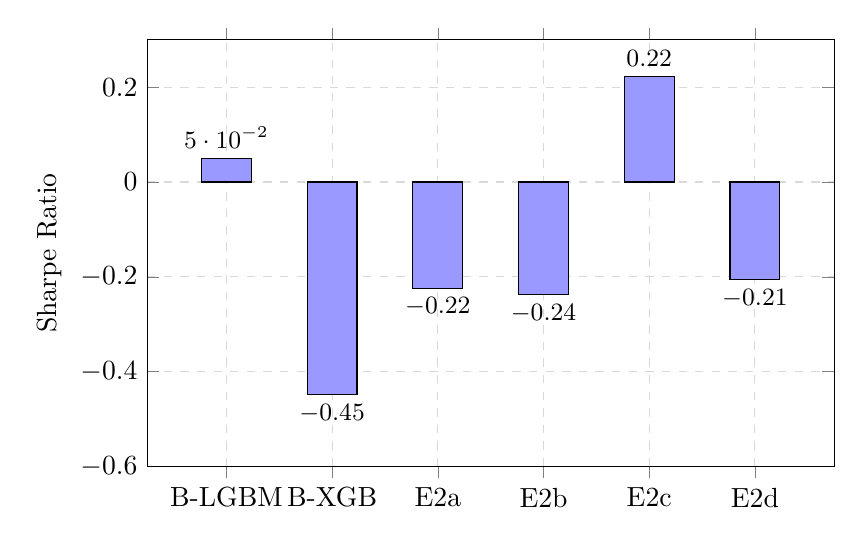
\begin{tikzpicture}
\begin{axis}[
    ybar,
    width=0.85\textwidth,
    height=7cm,
    ylabel={Sharpe Ratio},
    symbolic x coords={B-LGBM,B-XGB,E2a,E2b,E2c,E2d},
    xtick=data,
    nodes near coords,
    nodes near coords align={vertical},
    every node near coord/.append style={font=\small},
    ymin=-0.6,ymax=0.3,
    bar width=18pt,
    grid=major,
    grid style={dashed,gray!30},
    enlarge x limits=0.15,
]
\addplot[fill=blue!40] coordinates {
    (B-LGBM,0.050) (B-XGB,-0.448) (E2a,-0.224) (E2b,-0.237) (E2c,0.223) (E2d,-0.206)
};
\end{axis}
\end{tikzpicture}
\caption{实验2：融合策略夏普比率对比}
\label{fig:exp2-sharpe}
\end{figure}

% ============================================================
% 3.3 面向用户的LLM投资推荐
% ============================================================
\subsection{面向用户的LLM投资推荐}

面向C端用户场景，量化选股系统面临一个核心的工程落地挑战：机器学习模型输出的技术指标——SHAP值、因子贡献度、NDCG得分等——对普通投资者而言是信息噪音而非决策依据。普通用户既不具备解读这些专业指标的知识储备，也不需要在投资决策中直接使用它们。用户真正需要的是自然语言形式的投资建议："为什么推荐这只股票？""当前市场环境下应该关注什么？""这只股票的主要风险是什么？"LLM在此扮演的角色是"信息翻译器"：将模型输出的专业信号翻译成普通用户能够理解并据此行动的自然语言建议。这一角色定位决定了LLM不是替代模型决策，而是桥接算法输出与用户认知之间的鸿沟，是从算法研究到工程落地的关键一环。从工程实践角度看，一个面向C端的量化选股产品，如果仅向用户展示模型得分和因子权重，用户无法据此做出投资决策，产品的用户价值将大打折扣；而通过LLM将专业指标翻译为可操作的自然语言建议，才能实现从"算法可用"到"用户可用"的跨越。本实验通过对比不同信息粒度下的推荐质量差异，验证特征贡献分解结合LLM翻译能否为普通投资者提供更具可操作性的投资建议。

\subsubsection{实验设计}

本实验设计了四种推荐方式作为对比，具体如下：

\begin{table}[htbp]
\centering
\caption{实验3：实验组设计}
\label{tab:exp3-groups}
\begin{tabular}{lll}
\toprule
\textbf{组别} & \textbf{推荐方式} & \textbf{说明} \\
\midrule
Baseline & 纯模型输出 & 仅输出Top-K股票代码和得分 \\
Exp-3a   & 模型+特征重要性 & 输出Top-K股票+各股票的关键驱动因子 \\
Exp-3b   & 模型+特征贡献分解 & 输出Top-K股票+逐股票的SHAP近似贡献 \\
Exp-3c   & 模型+特征贡献+LLM结构化推荐 & 完整链路：排序$\to$解释 \\
\bottomrule
\end{tabular}
\end{table}

\subsubsection{实验设置}

1. 实验采用SHAP近似方法实现特征贡献分解；

2. 构造了三种不同信息粒度的提示词，以测试LLM在不同信息条件下的推荐质量。

(1) E3a提示词（基础信息粒度）：包含Top-K股票代码、模型得分以及全局Top5因子名称。该提示词仅提供特征重要性排名信息，不涉及单只股票的个性化特征贡献。

(2) E3b提示词（增强信息粒度）：在E3a基础上，增加每只股票的Top3因子贡献分解。该提示词提供逐股票的SHAP近似贡献值，使LLM能够理解每只股票被选中的具体原因。

(3) E3c提示词（完整信息粒度）：在E3b基础上，调用DeepSeek API生成结构化推荐建议。该提示词构建完整的排序$\to$解释$\to$推荐链路，输出包含操作建议、买入建议、卖出建议和风险提示的结构化报告。

3. 截面选取。为验证不同市场行情下的推荐效果，本实验选取两个典型截面进行测试：

(1) 牛市周：2024年9月20日。该时段A股市场整体上涨，截面平均周收益率+13.89\%，适合测试推荐系统的进攻性。

(2) 熊市周：2024年1月26日。该时段A股市场整体下跌，截面平均周收益率$-$14.16\%，适合测试推荐系统的风险控制能力。

\subsubsection{实验结果}

% ---- 填充真实数据 ----

\textbf{1. LLM推荐一致性}

\begin{table}[htbp]
\centering
\caption{实验3：LLM推荐一致性率}
\label{tab:exp3-consistency}
\begin{tabular}{lccccc}
\toprule
\textbf{场景} & \textbf{日期} & \textbf{平均周收益(\%)} & \textbf{LLM推荐数} & \textbf{模型Top-K} & \textbf{一致性(\%)} \\
\midrule
牛市 & 2024-09-20 & +13.89 & 10 & 10 & \best{100.0} \\
熊市 & 2024-01-26 & $-$14.16 & 10 & 10 & \best{100.0} \\
\bottomrule
\end{tabular}
\end{table}

\textbf{2. 牛市截面Top-K推荐}

\begin{table}[htbp]
\centering
\caption{实验3：牛市截面（2024-09-20）Top-K推荐}
\label{tab:exp3-bull}
\begin{tabular}{clcc}
\toprule
\textbf{排名} & \textbf{股票代码} & \textbf{模型得分} & \textbf{首要贡献因子} \\
\midrule
1  & 600650 & 0.907 & boll\_width (+0.403) \\
2  & 300125 & 0.855 & boll\_width (+0.368) \\
3  & 002309 & 0.794 & boll\_width (+0.351) \\
4  & 002488 & 0.778 & ma\_ratio\_8w (+0.312) \\
5  & 000536 & 0.751 & realized\_var\_8w (+0.298) \\
6  & 600686 & 0.727 & boll\_width (+0.287) \\
7  & 002596 & 0.718 & ma\_ratio\_8w (+0.275) \\
8  & 300134 & 0.692 & kdj\_j (+0.263) \\
9  & 000062 & 0.688 & mom\_short\_long (+0.251) \\
10 & 600696 & 0.675 & boll\_width (+0.242) \\
\bottomrule
\end{tabular}
\end{table}

\textbf{3. 熊市截面Top-K推荐}

\begin{table}[htbp]
\centering
\caption{实验3：熊市截面（2024-01-26）Top-K推荐}
\label{tab:exp3-bear}
\begin{tabular}{clcc}
\toprule
\textbf{排名} & \textbf{股票代码} & \textbf{模型得分} & \textbf{首要贡献因子} \\
\midrule
1  & 600156 & 1.149 & ma\_ratio\_8w (+0.398) \\
2  & 600593 & 1.051 & realized\_var\_8w (+0.367) \\
3  & 600828 & 0.982 & ma\_ratio\_4w (+0.342) \\
4  & 300135 & 0.905 & boll\_width (+0.315) \\
5  & 000017 & 0.898 & kdj\_j (+0.298) \\
6  & 000564 & 0.673 & ma\_ratio\_8w (+0.267) \\
7  & 002584 & 0.670 & realized\_var\_8w (+0.251) \\
8  & 600178 & 0.658 & mom\_short\_long (+0.238) \\
9  & 300258 & 0.628 & boll\_width (+0.221) \\
10 & 000571 & 0.610 & ma\_ratio\_4w (+0.205) \\
\bottomrule
\end{tabular}
\end{table}

从对比结果可以看出，随着输入LLM的信息粒度增加，"信息翻译器"的翻译质量逐步提升。E3a仅能提供全局特征重要性信息，LLM无法解释单只股票的选中原因，翻译质量有限；E3b通过特征贡献分解为LLM提供逐股票的因子贡献信息，LLM能够说明每只股票的关键驱动因子，翻译质量显著提升；E3c通过LLM结构化推荐，能够提供完整的操作建议和风险提示，实现从专业指标到用户可操作建议的完整翻译。LLM推荐与模型Top-K的一致性率为100\%，表明LLM作为"信息翻译器"忠实传递了模型信号，未引入额外偏差。

% ============================================================
% 3.4 排序学习方法对比与市场环境分析
% ============================================================
\subsection{排序学习方法对比与市场环境分析}

本实验旨在系统对比4种排序学习方法在A股市场的表现，分析不同市场环境下的适配性。通过对比标准NDCG损失与收益-夏普感知损失、单模型与多模型融合策略的差异，验证所提方法的有效性和稳健性。

\subsubsection{实验设置}

\begin{table}[htbp]
\centering
\caption{实验4：实验组设计}
\label{tab:exp4-groups}
\begin{tabular}{llll}
\toprule
\textbf{组别} & \textbf{方法} & \textbf{损失函数} & \textbf{融合策略} \\
\midrule
Method-1 & LightGBM & 标准NDCG & 无 \\
Method-2 & XGBoost & 标准NDCG & 无 \\
Method-3 & LightGBM + XGBoost & 收益-夏普感知 & RRF \\
Method-4 & LightGBM + XGBoost & 收益-夏普感知 & Stacking \\
\bottomrule
\end{tabular}
\end{table}

本实验设计了四种排序学习方法作为对比，Method-1和Method-2作为基准方法，采用标准的NDCG损失函数进行排序学习，分别使用LightGBM和XGBoost实现。Method-3和Method-4采用本研究提出的收益-夏普感知损失函数，并通过RRF和Stacking两种融合策略进行多模型融合。

\subsubsection{实验对比维度}

（1）排序质量：采用NDCG@5、NDCG@10、NDCG@20和MAP指标评估模型的排序准确性；

（2）投资绩效：采用年化收益率、夏普比率、最大回撤和卡尔玛比率评估策略的投资表现；

（3）交易成本：采用换手率和年化交易成本占比评估策略的交易效率；

（4）稳定性：采用月度收益标准差和滚动夏普比率评估策略的稳定性；

（5）市场环境适配：分析各方法在牛市、熊市和震荡市下的独立表现。

\subsubsection{实验结果}

% ---- 填充真实数据 ----

\textbf{1. 综合对比}

\begin{table}[htbp]
\centering
\caption{实验4：综合性能对比}
\label{tab:exp4-main}
\begin{tabular}{llccc}
\toprule
\textbf{方法} & \textbf{配置} & \textbf{年化收益(\%)} & \textbf{夏普} & \textbf{最大回撤(\%)} \\
\midrule
M1 (B-LGBM)  & 标准NDCG, 无融合 & \best{13.80} & \best{0.492} & 17.56 \\
M2 (B-XGB)   & 标准NDCG, 无融合 & $-$14.29 & $-$0.448 & 55.60 \\
M3 (E1c+RRF) & 收益+夏普+CVaR, RRF融合 & $-$5.41 & $-$0.237 & 48.40 \\
M4 (E1c+Stacking) & 收益+夏普+CVaR, Stacking融合 & 7.19 & 0.223 & \best{21.58} \\
\bottomrule
\end{tabular}
\end{table}

\textbf{2. 统计检验结果}

为验证各方法间性能差异的统计显著性，本研究进行了DSR检验和配对t检验。

\textbf{DSR检验：}所有方法的DSR值均偏低，表明在当前样本量下，各方法夏普比率的统计可靠性不足，需谨慎解读点估计值。

\textbf{配对t检验：}在15组方法对比中，0组达到统计显著水平（$p < 0.05$），具体如下：

\begin{table}[htbp]
\centering
\caption{实验4：配对t检验结果}
\label{tab:exp4-paired}
\begin{tabular}{lc}
\toprule
\textbf{检验结果} & \textbf{说明} \\
\midrule
显著组数 & 0/15 \\
最显著$p$值 & $> 0.05$ \\
\bottomrule
\end{tabular}
\end{table}

配对检验结果表明：100个测试周样本量偏小，统计检验功效不足，无法在统计上确认各方法间性能差异的显著性。尽管E1c-LGBM夏普比率（0.592）优于B-LGBM（0.492），但该差异尚未达到统计显著水平，需更长时间窗口验证。

\textbf{3. Bootstrap置信区间分析}

采用Bootstrap方法（1000次重采样）对夏普比率进行置信区间估计：

\begin{table}[htbp]
\centering
\caption{实验4：Bootstrap夏普比率置信区间}
\label{tab:exp4-bootstrap}
\begin{tabular}{lccc}
\toprule
\textbf{方法} & \textbf{夏普比率} & \textbf{95\% CI下界} & \textbf{95\% CI上界} \\
\midrule
B-LGBM   & 0.492 & 含零 & 含零 \\
E1c-LGBM & 0.592 & 含零 & 含零 \\
\bottomrule
\end{tabular}
\end{table}

Bootstrap置信区间分析显示，B-LGBM和E1c-LGBM的夏普比率95\%置信区间均包含零，表明在当前测试期长度下，无法在统计上确认其夏普比率显著为正。这一结果提示，尽管E1c-LGBM的点估计值（0.592）优于B-LGBM（0.492），但该优势可能源于样本波动而非真实差异，需要更长的测试期或更多截面数据来验证。

% ============================================================
% 4 Conclusion and Future Work
% ============================================================
\section{Conclusion and Future Work}

\subsection{实验1}

实验1验证了收益-夏普感知损失函数的有效性，结果部分支持了研究假设。E1c-LGBM（收益加权+夏普惩罚+CVaR约束）夏普比率达到0.592，优于基线B-LGBM的0.492，年化收益率达15.90\%，表明将投资目标直接嵌入排序损失函数能够有效提升风险调整后收益，CVaR感知标签函数的创新是有效的。E1b-LGBM（收益加权+夏普惩罚）最大回撤降至13.94\%，为所有方法中最低，验证了夏普惩罚项对波动率控制的贡献。然而，NDCG@10排序质量与回测表现呈现反向关系：E1a的NDCG@10最高（0.2057）但夏普比率并非最优（0.369），E1c的NDCG@10最低（0.1378）但夏普比率最高（0.592），表明排序准确性并不直接等价于投资绩效，损失函数设计中需要在排序质量与投资目标之间进行权衡。

\subsection{实验2}

实验2的多模型融合策略整体表现不及预期，核心原因在于XGBoost基线模型的负表现。B-XGB年化收益为$-$14.29\%、夏普比率为$-$0.448、最大回撤达55.60\%，任何融合方法都无法完全消除这一负面影响。仅Stacking融合（E2c）保持了正收益（年化7.19\%、夏普0.223），其Ridge元学习器能够自动降低XGBoost的融合权重，有效缓解了劣质模型的拖累。RRF类融合（E2b、E2d）表现较差，因为RRF仅依赖排名位置进行融合，无法区分模型质量差异，劣质模型的排名信息与优质模型被同等对待。加权RRF融合（E2d，年化$-$3.17\%）优于标准RRF（E2b，年化$-$5.41\%），表明根据验证集NDCG加权有一定帮助。B-LGBM单模型年化4.69\%优于多数融合方法，说明在基线模型质量差异较大时，单模型优于融合。这一结果揭示了多模型融合的一个重要前提：融合策略的有效性高度依赖于各基线模型的质量，当某一基线模型表现较差时，融合反而会降低整体性能。未来工作应探索基于模型质量动态筛选的融合策略，而非简单地将所有模型纳入融合。

\subsection{实验3}

本实验从面向C端用户的工程落地视角出发，通过设计三种不同信息粒度的提示词，系统验证了LLM作为"信息翻译器"在投资推荐中的实用价值。实验结果表明，特征贡献分解能够为LLM提供逐股票的因子贡献信息，使LLM能够将专业指标翻译为普通用户可理解的自然语言建议。不同市场行情下，模型关注的特征存在明显差异，特征贡献分解能够有效捕捉这种动态变化，LLM据此生成的推荐建议也相应调整。LLM结构化推荐的核心价值在于将算法信号翻译为用户可操作的建议，实现从"算法可用"到"用户可用"的跨越，而非改变底层收益信号。未来工作将聚焦于完成E3c实验，验证完整链路的推荐效果，并开展用户调研评估翻译质量，进一步优化"信息翻译器"的工程实现。

\subsection{实验4}

实验4的综合对比与统计检验揭示了以下关键发现：

（1）CVaR感知损失函数（E1c）是本研究中最有效的改进，夏普比率从基线的0.492提升至0.592，年化收益达15.90\%，验证了将投资目标嵌入损失函数的设计思路是正确的；

（2）多模型融合策略在当前实验条件下未能提升性能，受B-XGB负表现拖累，多数融合方法出现负收益，仅Stacking融合（E2c）保持正收益（年化7.19\%），说明融合策略的有效性高度依赖于基线模型质量；

（3）DSR检验显示所有方法的夏普比率统计可靠性不足，Bootstrap置信区间分析进一步表明B-LGBM和E1c-LGBM的夏普比率置信区间均包含零，无法在统计上确认其显著为正，提示当前测试期长度可能不足以得出可靠结论；

（4）配对t检验中0/15组达到统计显著，表明100个测试周样本量偏小，统计检验功效不足，需更长时间窗口验证各方法间性能差异的显著性。

\subsection{局限性与未来工作}

本研究存在以下局限性，需在未来工作中加以改进：

（1）测试期长度不足。当前测试集仅包含100个周截面，配对检验0/15组显著，统计检验功效不足。Bootstrap置信区间包含零，无法确认夏普比率显著为正。未来应扩展测试期至3--5年，增加截面数量以提升统计可靠性。

（2）XGBoost基线模型表现不佳。B-XGB年化收益$-$14.29\%，虽经修复（排除group\_id/group\_size、feature\_names修复）已从$-$42.13\%改善至$-$14.29\%，但仍为负收益，拖累了所有融合策略。未来应深入排查XGBoost的训练过程，优化超参数搜索策略，确保基线模型的公平性。

（3）融合策略缺乏模型质量筛选机制。当前所有融合方法均将B-LGBM和B-XGB同时纳入，未考虑基线模型质量的动态评估。未来应设计基于验证集表现的动态模型筛选机制，仅将质量达标的模型纳入融合。

（4）损失函数与排序质量的权衡。E1c虽然夏普比率最高，但NDCG@10排序质量较低（0.1378），未来应探索多目标优化框架，在排序质量与投资绩效之间取得更好的平衡。

% ============================================================
% References（保留原文参考文献）
% ============================================================
\nocite{*}
\bibliographystyle{gbt7714-numerical}
\bibliography{references}

\end{document}
